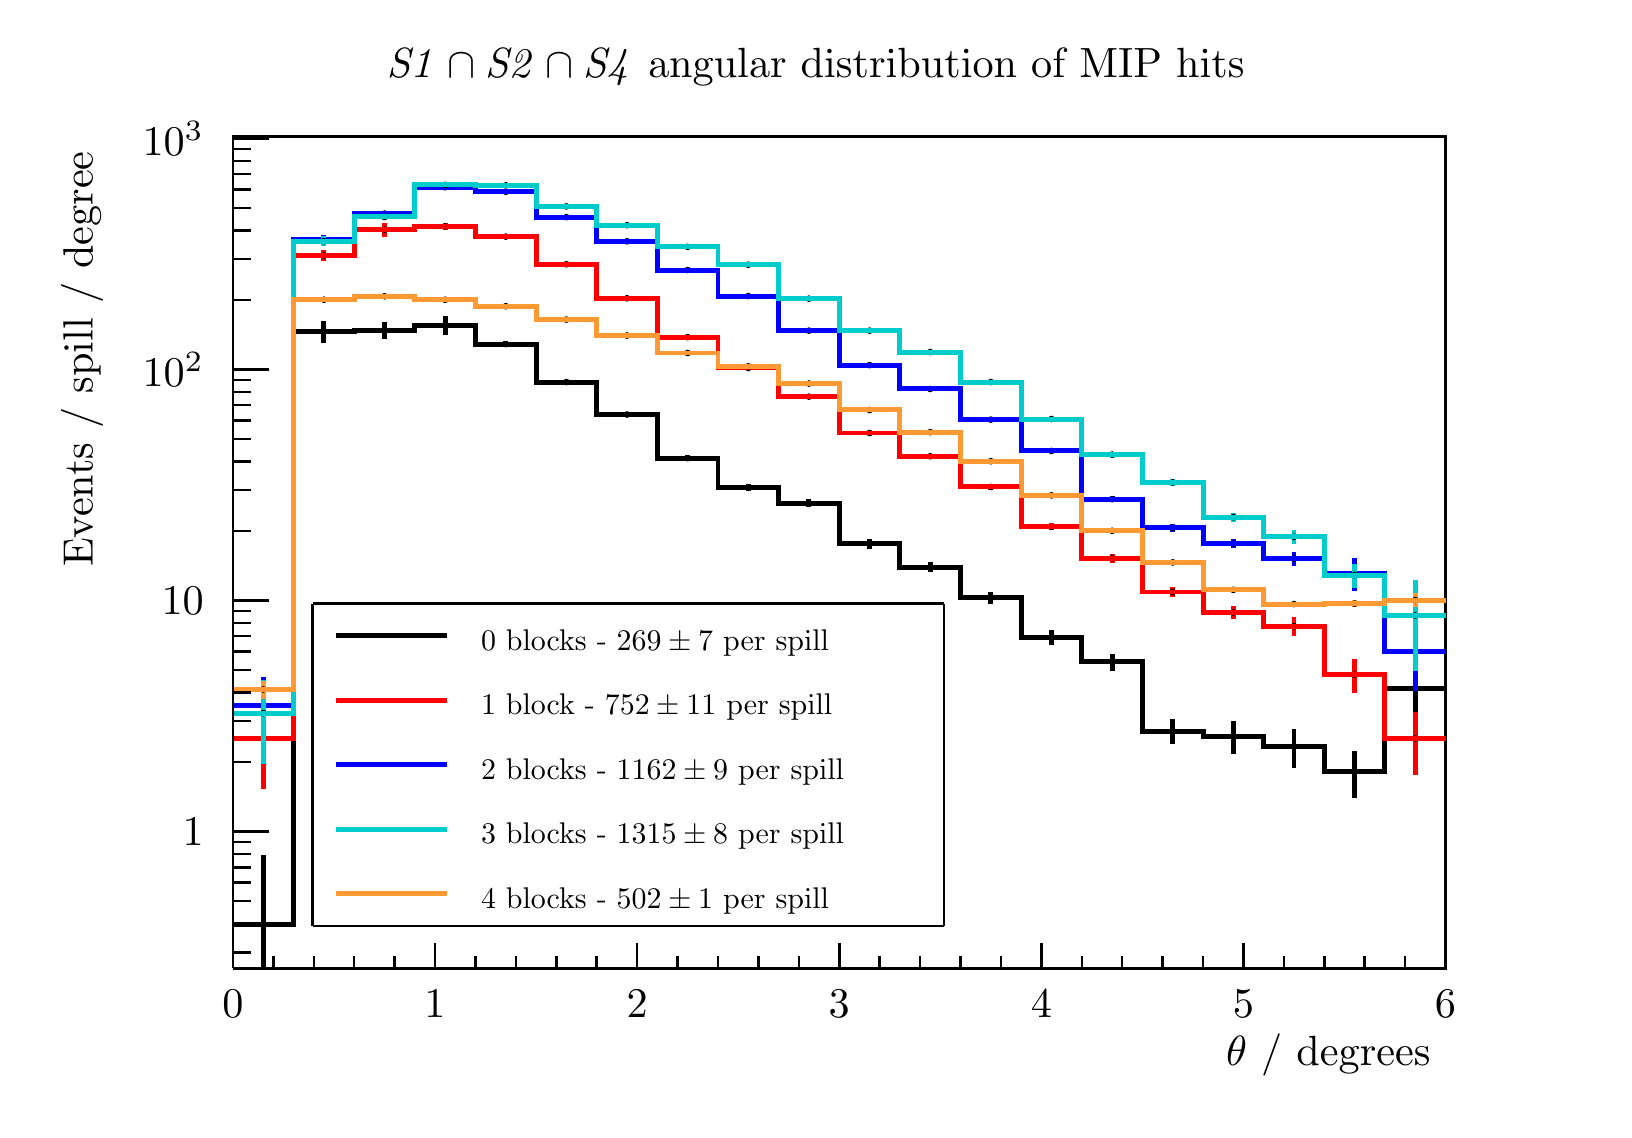
\begin{tikzpicture}
\pgfdeclareplotmark{cross} {
\pgfpathmoveto{\pgfpoint{-0.3\pgfplotmarksize}{\pgfplotmarksize}}
\pgfpathlineto{\pgfpoint{+0.3\pgfplotmarksize}{\pgfplotmarksize}}
\pgfpathlineto{\pgfpoint{+0.3\pgfplotmarksize}{0.3\pgfplotmarksize}}
\pgfpathlineto{\pgfpoint{+1\pgfplotmarksize}{0.3\pgfplotmarksize}}
\pgfpathlineto{\pgfpoint{+1\pgfplotmarksize}{-0.3\pgfplotmarksize}}
\pgfpathlineto{\pgfpoint{+0.3\pgfplotmarksize}{-0.3\pgfplotmarksize}}
\pgfpathlineto{\pgfpoint{+0.3\pgfplotmarksize}{-1.\pgfplotmarksize}}
\pgfpathlineto{\pgfpoint{-0.3\pgfplotmarksize}{-1.\pgfplotmarksize}}
\pgfpathlineto{\pgfpoint{-0.3\pgfplotmarksize}{-0.3\pgfplotmarksize}}
\pgfpathlineto{\pgfpoint{-1.\pgfplotmarksize}{-0.3\pgfplotmarksize}}
\pgfpathlineto{\pgfpoint{-1.\pgfplotmarksize}{0.3\pgfplotmarksize}}
\pgfpathlineto{\pgfpoint{-0.3\pgfplotmarksize}{0.3\pgfplotmarksize}}
\pgfpathclose
\pgfusepathqstroke
}
\pgfdeclareplotmark{cross*} {
\pgfpathmoveto{\pgfpoint{-0.3\pgfplotmarksize}{\pgfplotmarksize}}
\pgfpathlineto{\pgfpoint{+0.3\pgfplotmarksize}{\pgfplotmarksize}}
\pgfpathlineto{\pgfpoint{+0.3\pgfplotmarksize}{0.3\pgfplotmarksize}}
\pgfpathlineto{\pgfpoint{+1\pgfplotmarksize}{0.3\pgfplotmarksize}}
\pgfpathlineto{\pgfpoint{+1\pgfplotmarksize}{-0.3\pgfplotmarksize}}
\pgfpathlineto{\pgfpoint{+0.3\pgfplotmarksize}{-0.3\pgfplotmarksize}}
\pgfpathlineto{\pgfpoint{+0.3\pgfplotmarksize}{-1.\pgfplotmarksize}}
\pgfpathlineto{\pgfpoint{-0.3\pgfplotmarksize}{-1.\pgfplotmarksize}}
\pgfpathlineto{\pgfpoint{-0.3\pgfplotmarksize}{-0.3\pgfplotmarksize}}
\pgfpathlineto{\pgfpoint{-1.\pgfplotmarksize}{-0.3\pgfplotmarksize}}
\pgfpathlineto{\pgfpoint{-1.\pgfplotmarksize}{0.3\pgfplotmarksize}}
\pgfpathlineto{\pgfpoint{-0.3\pgfplotmarksize}{0.3\pgfplotmarksize}}
\pgfpathclose
\pgfusepathqfillstroke
}
\pgfdeclareplotmark{newstar} {
\pgfpathmoveto{\pgfqpoint{0pt}{\pgfplotmarksize}}
\pgfpathlineto{\pgfqpointpolar{44}{0.5\pgfplotmarksize}}
\pgfpathlineto{\pgfqpointpolar{18}{\pgfplotmarksize}}
\pgfpathlineto{\pgfqpointpolar{-20}{0.5\pgfplotmarksize}}
\pgfpathlineto{\pgfqpointpolar{-54}{\pgfplotmarksize}}
\pgfpathlineto{\pgfqpointpolar{-90}{0.5\pgfplotmarksize}}
\pgfpathlineto{\pgfqpointpolar{234}{\pgfplotmarksize}}
\pgfpathlineto{\pgfqpointpolar{198}{0.5\pgfplotmarksize}}
\pgfpathlineto{\pgfqpointpolar{162}{\pgfplotmarksize}}
\pgfpathlineto{\pgfqpointpolar{134}{0.5\pgfplotmarksize}}
\pgfpathclose
\pgfusepathqstroke
}
\pgfdeclareplotmark{newstar*} {
\pgfpathmoveto{\pgfqpoint{0pt}{\pgfplotmarksize}}
\pgfpathlineto{\pgfqpointpolar{44}{0.5\pgfplotmarksize}}
\pgfpathlineto{\pgfqpointpolar{18}{\pgfplotmarksize}}
\pgfpathlineto{\pgfqpointpolar{-20}{0.5\pgfplotmarksize}}
\pgfpathlineto{\pgfqpointpolar{-54}{\pgfplotmarksize}}
\pgfpathlineto{\pgfqpointpolar{-90}{0.5\pgfplotmarksize}}
\pgfpathlineto{\pgfqpointpolar{234}{\pgfplotmarksize}}
\pgfpathlineto{\pgfqpointpolar{198}{0.5\pgfplotmarksize}}
\pgfpathlineto{\pgfqpointpolar{162}{\pgfplotmarksize}}
\pgfpathlineto{\pgfqpointpolar{134}{0.5\pgfplotmarksize}}
\pgfpathclose
\pgfusepathqfillstroke
}
\definecolor{c}{rgb}{1,1,1};
\draw [color=c, fill=c] (0,0) rectangle (20,13.7249);
\draw [color=c, fill=c] (2.6,1.78424) rectangle (18,12.3524);
\definecolor{c}{rgb}{0,0,0};
\draw [c,line width=0.9] (2.6,1.78424) -- (2.6,12.3524) -- (18,12.3524) -- (18,1.78424) -- (2.6,1.78424);
\definecolor{c}{rgb}{1,1,1};
\draw [color=c, fill=c] (2.6,1.78424) rectangle (18,12.3524);
\definecolor{c}{rgb}{0,0,0};
\draw [c,line width=0.9] (2.6,1.78424) -- (2.6,12.3524) -- (18,12.3524) -- (18,1.78424) -- (2.6,1.78424);
\definecolor{c}{rgb}{0,0,0.6};
\draw [c,line width=0.9] (2.6,1.78424) -- (3.37,1.78424) -- (3.37,1.78424) -- (4.14,1.78424) -- (4.14,1.78424) -- (4.91,1.78424) -- (4.91,1.78424) -- (5.68,1.78424) -- (5.68,1.78424) -- (6.45,1.78424) -- (6.45,1.78424) -- (7.22,1.78424) --
 (7.22,1.78424) -- (7.99,1.78424) -- (7.99,1.78424) -- (8.76,1.78424) -- (8.76,1.78424) -- (9.53,1.78424) -- (9.53,1.78424) -- (10.3,1.78424) -- (10.3,1.78424) -- (11.07,1.78424) -- (11.07,1.78424) -- (11.84,1.78424) -- (11.84,1.78424) --
 (12.61,1.78424) -- (12.61,1.78424) -- (13.38,1.78424) -- (13.38,1.78424) -- (14.15,1.78424) -- (14.15,1.78424) -- (14.92,1.78424) -- (14.92,1.78424) -- (15.69,1.78424) -- (15.69,1.78424) -- (16.46,1.78424) -- (16.46,1.78424) -- (17.23,1.78424) --
 (17.23,1.78424) -- (18,1.78424);
\definecolor{c}{rgb}{0,0,0};
\draw [c,line width=0.9] (2.6,1.78424) -- (18,1.78424);
\draw [c,line width=0.9] (2.6,2.10129) -- (2.6,1.78424);
\draw [c,line width=0.9] (3.11333,1.94276) -- (3.11333,1.78424);
\draw [c,line width=0.9] (3.62667,1.94276) -- (3.62667,1.78424);
\draw [c,line width=0.9] (4.14,1.94276) -- (4.14,1.78424);
\draw [c,line width=0.9] (4.65333,1.94276) -- (4.65333,1.78424);
\draw [c,line width=0.9] (5.16667,2.10129) -- (5.16667,1.78424);
\draw [c,line width=0.9] (5.68,1.94276) -- (5.68,1.78424);
\draw [c,line width=0.9] (6.19333,1.94276) -- (6.19333,1.78424);
\draw [c,line width=0.9] (6.70667,1.94276) -- (6.70667,1.78424);
\draw [c,line width=0.9] (7.22,1.94276) -- (7.22,1.78424);
\draw [c,line width=0.9] (7.73333,2.10129) -- (7.73333,1.78424);
\draw [c,line width=0.9] (8.24667,1.94276) -- (8.24667,1.78424);
\draw [c,line width=0.9] (8.76,1.94276) -- (8.76,1.78424);
\draw [c,line width=0.9] (9.27333,1.94276) -- (9.27333,1.78424);
\draw [c,line width=0.9] (9.78667,1.94276) -- (9.78667,1.78424);
\draw [c,line width=0.9] (10.3,2.10129) -- (10.3,1.78424);
\draw [c,line width=0.9] (10.8133,1.94276) -- (10.8133,1.78424);
\draw [c,line width=0.9] (11.3267,1.94276) -- (11.3267,1.78424);
\draw [c,line width=0.9] (11.84,1.94276) -- (11.84,1.78424);
\draw [c,line width=0.9] (12.3533,1.94276) -- (12.3533,1.78424);
\draw [c,line width=0.9] (12.8667,2.10129) -- (12.8667,1.78424);
\draw [c,line width=0.9] (13.38,1.94276) -- (13.38,1.78424);
\draw [c,line width=0.9] (13.8933,1.94276) -- (13.8933,1.78424);
\draw [c,line width=0.9] (14.4067,1.94276) -- (14.4067,1.78424);
\draw [c,line width=0.9] (14.92,1.94276) -- (14.92,1.78424);
\draw [c,line width=0.9] (15.4333,2.10129) -- (15.4333,1.78424);
\draw [c,line width=0.9] (15.9467,1.94276) -- (15.9467,1.78424);
\draw [c,line width=0.9] (16.46,1.94276) -- (16.46,1.78424);
\draw [c,line width=0.9] (16.9733,1.94276) -- (16.9733,1.78424);
\draw [c,line width=0.9] (17.4867,1.94276) -- (17.4867,1.78424);
\draw [c,line width=0.9] (18,2.10129) -- (18,1.78424);
\draw [anchor=base] (2.6,1.16662) node[scale=1.52731, color=c, rotate=0]{0};
\draw [anchor=base] (5.16667,1.16662) node[scale=1.52731, color=c, rotate=0]{1};
\draw [anchor=base] (7.73333,1.16662) node[scale=1.52731, color=c, rotate=0]{2};
\draw [anchor=base] (10.3,1.16662) node[scale=1.52731, color=c, rotate=0]{3};
\draw [anchor=base] (12.8667,1.16662) node[scale=1.52731, color=c, rotate=0]{4};
\draw [anchor=base] (15.4333,1.16662) node[scale=1.52731, color=c, rotate=0]{5};
\draw [anchor=base] (18,1.16662) node[scale=1.52731, color=c, rotate=0]{6};
\draw [anchor= east] (18,0.686246) node[scale=1.52731, color=c, rotate=0]{$ \theta$ / degrees};
\draw [c,line width=0.9] (2.6,1.78424) -- (2.6,12.3524);
\draw [c,line width=0.9] (2.831,1.98949) -- (2.6,1.98949);
\draw [c,line width=0.9] (2.831,2.35605) -- (2.6,2.35605);
\draw [c,line width=0.9] (2.831,2.64038) -- (2.6,2.64038);
\draw [c,line width=0.9] (2.831,2.87269) -- (2.6,2.87269);
\draw [c,line width=0.9] (2.831,3.06911) -- (2.6,3.06911);
\draw [c,line width=0.9] (2.831,3.23925) -- (2.6,3.23925);
\draw [c,line width=0.9] (2.831,3.38933) -- (2.6,3.38933);
\draw [c,line width=0.9] (3.062,3.52358) -- (2.6,3.52358);
\draw [anchor= east] (2.42,3.52358) node[scale=1.52731, color=c, rotate=0]{1};
\draw [c,line width=0.9] (2.831,4.40678) -- (2.6,4.40678);
\draw [c,line width=0.9] (2.831,4.92342) -- (2.6,4.92342);
\draw [c,line width=0.9] (2.831,5.28998) -- (2.6,5.28998);
\draw [c,line width=0.9] (2.831,5.57431) -- (2.6,5.57431);
\draw [c,line width=0.9] (2.831,5.80662) -- (2.6,5.80662);
\draw [c,line width=0.9] (2.831,6.00304) -- (2.6,6.00304);
\draw [c,line width=0.9] (2.831,6.17318) -- (2.6,6.17318);
\draw [c,line width=0.9] (2.831,6.32326) -- (2.6,6.32326);
\draw [c,line width=0.9] (3.062,6.45751) -- (2.6,6.45751);
\draw [anchor= east] (2.42,6.45751) node[scale=1.52731, color=c, rotate=0]{10};
\draw [c,line width=0.9] (2.831,7.34071) -- (2.6,7.34071);
\draw [c,line width=0.9] (2.831,7.85735) -- (2.6,7.85735);
\draw [c,line width=0.9] (2.831,8.22391) -- (2.6,8.22391);
\draw [c,line width=0.9] (2.831,8.50824) -- (2.6,8.50824);
\draw [c,line width=0.9] (2.831,8.74055) -- (2.6,8.74055);
\draw [c,line width=0.9] (2.831,8.93697) -- (2.6,8.93697);
\draw [c,line width=0.9] (2.831,9.10711) -- (2.6,9.10711);
\draw [c,line width=0.9] (2.831,9.25719) -- (2.6,9.25719);
\draw [c,line width=0.9] (3.062,9.39144) -- (2.6,9.39144);
\draw [anchor= east] (2.42,9.39144) node[scale=1.52731, color=c, rotate=0]{$10^{2}$};
\draw [c,line width=0.9] (2.831,10.2746) -- (2.6,10.2746);
\draw [c,line width=0.9] (2.831,10.7913) -- (2.6,10.7913);
\draw [c,line width=0.9] (2.831,11.1578) -- (2.6,11.1578);
\draw [c,line width=0.9] (2.831,11.4422) -- (2.6,11.4422);
\draw [c,line width=0.9] (2.831,11.6745) -- (2.6,11.6745);
\draw [c,line width=0.9] (2.831,11.8709) -- (2.6,11.8709);
\draw [c,line width=0.9] (2.831,12.041) -- (2.6,12.041);
\draw [c,line width=0.9] (2.831,12.1911) -- (2.6,12.1911);
\draw [c,line width=0.9] (3.062,12.3254) -- (2.6,12.3254);
\draw [anchor= east] (2.42,12.3254) node[scale=1.52731, color=c, rotate=0]{$10^{3}$};
\draw [anchor= east] (0.683095,12.3524) node[scale=1.52731, color=c, rotate=90]{ Events / spill / degree};
\draw [c,line width=1.8] (2.985,1.78424) -- (2.985,2.34153);
\draw [c,line width=1.8] (2.985,2.34153) -- (2.985,3.22749);
\foreach \P in {(2.985,2.34153)}{\draw[mark options={color=c,fill=c},mark size=2.402402pt,mark=*,mark size=1pt] plot coordinates {\P};}
\draw [c,line width=1.8] (3.755,9.73343) -- (3.755,9.8787);
\draw [c,line width=1.8] (3.755,9.8787) -- (3.755,10.0091);
\foreach \P in {(3.755,9.8787)}{\draw[mark options={color=c,fill=c},mark size=2.402402pt,mark=*,mark size=1pt] plot coordinates {\P};}
\draw [c,line width=1.8] (4.525,9.7762) -- (4.525,9.88687);
\draw [c,line width=1.8] (4.525,9.88687) -- (4.525,9.98869);
\foreach \P in {(4.525,9.88687)}{\draw[mark options={color=c,fill=c},mark size=2.402402pt,mark=*,mark size=1pt] plot coordinates {\P};}
\draw [c,line width=1.8] (5.295,9.82881) -- (5.295,9.95409);
\draw [c,line width=1.8] (5.295,9.95409) -- (5.295,10.0681);
\foreach \P in {(5.295,9.95409)}{\draw[mark options={color=c,fill=c},mark size=2.402402pt,mark=*,mark size=1pt] plot coordinates {\P};}
\draw [c,line width=1.8] (6.065,9.67782) -- (6.065,9.71317);
\draw [c,line width=1.8] (6.065,9.71317) -- (6.065,9.74756);
\foreach \P in {(6.065,9.71317)}{\draw[mark options={color=c,fill=c},mark size=2.402402pt,mark=*,mark size=1pt] plot coordinates {\P};}
\draw [c,line width=1.8] (6.835,9.19869) -- (6.835,9.23103);
\draw [c,line width=1.8] (6.835,9.23103) -- (6.835,9.26256);
\foreach \P in {(6.835,9.23103)}{\draw[mark options={color=c,fill=c},mark size=2.402402pt,mark=*,mark size=1pt] plot coordinates {\P};}
\draw [c,line width=1.8] (7.605,8.78432) -- (7.605,8.81859);
\draw [c,line width=1.8] (7.605,8.81859) -- (7.605,8.85196);
\foreach \P in {(7.605,8.81859)}{\draw[mark options={color=c,fill=c},mark size=2.402402pt,mark=*,mark size=1pt] plot coordinates {\P};}
\draw [c,line width=1.8] (8.375,8.22429) -- (8.375,8.26496);
\draw [c,line width=1.8] (8.375,8.26496) -- (8.375,8.30436);
\foreach \P in {(8.375,8.26496)}{\draw[mark options={color=c,fill=c},mark size=2.402402pt,mark=*,mark size=1pt] plot coordinates {\P};}
\draw [c,line width=1.8] (9.145,7.84222) -- (9.145,7.88855);
\draw [c,line width=1.8] (9.145,7.88855) -- (9.145,7.93326);
\foreach \P in {(9.145,7.88855)}{\draw[mark options={color=c,fill=c},mark size=2.402402pt,mark=*,mark size=1pt] plot coordinates {\P};}
\draw [c,line width=1.8] (9.915,7.64411) -- (9.915,7.69365);
\draw [c,line width=1.8] (9.915,7.69365) -- (9.915,7.74133);
\foreach \P in {(9.915,7.69365)}{\draw[mark options={color=c,fill=c},mark size=2.402402pt,mark=*,mark size=1pt] plot coordinates {\P};}
\draw [c,line width=1.8] (10.685,7.11687) -- (10.685,7.17797);
\draw [c,line width=1.8] (10.685,7.17797) -- (10.685,7.23626);
\foreach \P in {(10.685,7.17797)}{\draw[mark options={color=c,fill=c},mark size=2.402402pt,mark=*,mark size=1pt] plot coordinates {\P};}
\draw [c,line width=1.8] (11.455,6.81446) -- (11.455,6.88113);
\draw [c,line width=1.8] (11.455,6.88113) -- (11.455,6.94449);
\foreach \P in {(11.455,6.88113)}{\draw[mark options={color=c,fill=c},mark size=2.402402pt,mark=*,mark size=1pt] plot coordinates {\P};}
\draw [c,line width=1.8] (12.225,6.41042) -- (12.225,6.48936);
\draw [c,line width=1.8] (12.225,6.48936) -- (12.225,6.5637);
\foreach \P in {(12.225,6.48936)}{\draw[mark options={color=c,fill=c},mark size=2.402402pt,mark=*,mark size=1pt] plot coordinates {\P};}
\draw [c,line width=1.8] (12.995,5.89235) -- (12.995,5.98953);
\draw [c,line width=1.8] (12.995,5.98953) -- (12.995,6.07983);
\foreach \P in {(12.995,5.98953)}{\draw[mark options={color=c,fill=c},mark size=2.402402pt,mark=*,mark size=1pt] plot coordinates {\P};}
\draw [c,line width=1.8] (13.765,5.56498) -- (13.765,5.67796);
\draw [c,line width=1.8] (13.765,5.67796) -- (13.765,5.78173);
\foreach \P in {(13.765,5.67796)}{\draw[mark options={color=c,fill=c},mark size=2.402402pt,mark=*,mark size=1pt] plot coordinates {\P};}
\draw [c,line width=1.8] (14.535,4.63213) -- (14.535,4.79858);
\draw [c,line width=1.8] (14.535,4.79858) -- (14.535,4.94578);
\foreach \P in {(14.535,4.79858)}{\draw[mark options={color=c,fill=c},mark size=2.402402pt,mark=*,mark size=1pt] plot coordinates {\P};}
\draw [c,line width=1.8] (15.305,4.50141) -- (15.305,4.73201);
\draw [c,line width=1.8] (15.305,4.73201) -- (15.305,4.9272);
\foreach \P in {(15.305,4.73201)}{\draw[mark options={color=c,fill=c},mark size=2.402402pt,mark=*,mark size=1pt] plot coordinates {\P};}
\draw [c,line width=1.8] (16.075,4.33584) -- (16.075,4.60575);
\draw [c,line width=1.8] (16.075,4.60575) -- (16.075,4.82836);
\foreach \P in {(16.075,4.60575)}{\draw[mark options={color=c,fill=c},mark size=2.402402pt,mark=*,mark size=1pt] plot coordinates {\P};}
\draw [c,line width=1.8] (16.845,3.94886) -- (16.845,4.2854);
\draw [c,line width=1.8] (16.845,4.2854) -- (16.845,4.55137);
\foreach \P in {(16.845,4.2854)}{\draw[mark options={color=c,fill=c},mark size=2.402402pt,mark=*,mark size=1pt] plot coordinates {\P};}
\draw [c,line width=1.8] (17.615,4.4306) -- (17.615,5.33657);
\draw [c,line width=1.8] (17.615,5.33657) -- (17.615,5.86071);
\foreach \P in {(17.615,5.33657)}{\draw[mark options={color=c,fill=c},mark size=2.402402pt,mark=*,mark size=1pt] plot coordinates {\P};}
\draw [c,line width=1.8] (2.6,2.34153) -- (3.37,2.34153) -- (3.37,9.8787) -- (4.14,9.8787) -- (4.14,9.88687) -- (4.91,9.88687) -- (4.91,9.95409) -- (5.68,9.95409) -- (5.68,9.71317) -- (6.45,9.71317) -- (6.45,9.23103) -- (7.22,9.23103) --
 (7.22,8.81859) -- (7.99,8.81859) -- (7.99,8.26496) -- (8.76,8.26496) -- (8.76,7.88855) -- (9.53,7.88855) -- (9.53,7.69365) -- (10.3,7.69365) -- (10.3,7.17797) -- (11.07,7.17797) -- (11.07,6.88113) -- (11.84,6.88113) -- (11.84,6.48936) --
 (12.61,6.48936) -- (12.61,5.98953) -- (13.38,5.98953) -- (13.38,5.67796) -- (14.15,5.67796) -- (14.15,4.79858) -- (14.92,4.79858) -- (14.92,4.73201) -- (15.69,4.73201) -- (15.69,4.60575) -- (16.46,4.60575) -- (16.46,4.2854) -- (17.23,4.2854) --
 (17.23,5.33657) -- (18,5.33657);
\definecolor{c}{rgb}{1,0,0};
\draw [c,line width=1.8] (2.985,4.06376) -- (2.985,4.70305);
\draw [c,line width=1.8] (2.985,4.70305) -- (2.985,5.12677);
\definecolor{c}{rgb}{0,0,0};
\foreach \P in {(2.985,4.70305)}{\draw[mark options={color=c,fill=c},mark size=2.402402pt,mark=*,mark size=1pt] plot coordinates {\P};}
\definecolor{c}{rgb}{1,0,0};
\draw [c,line width=1.8] (3.755,10.7639) -- (3.755,10.838);
\draw [c,line width=1.8] (3.755,10.838) -- (3.755,10.908);
\definecolor{c}{rgb}{0,0,0};
\foreach \P in {(3.755,10.838)}{\draw[mark options={color=c,fill=c},mark size=2.402402pt,mark=*,mark size=1pt] plot coordinates {\P};}
\definecolor{c}{rgb}{1,0,0};
\draw [c,line width=1.8] (4.525,11.0712) -- (4.525,11.1675);
\draw [c,line width=1.8] (4.525,11.1675) -- (4.525,11.2571);
\definecolor{c}{rgb}{0,0,0};
\foreach \P in {(4.525,11.1675)}{\draw[mark options={color=c,fill=c},mark size=2.402402pt,mark=*,mark size=1pt] plot coordinates {\P};}
\definecolor{c}{rgb}{1,0,0};
\draw [c,line width=1.8] (5.295,11.1634) -- (5.295,11.2076);
\draw [c,line width=1.8] (5.295,11.2076) -- (5.295,11.2503);
\definecolor{c}{rgb}{0,0,0};
\foreach \P in {(5.295,11.2076)}{\draw[mark options={color=c,fill=c},mark size=2.402402pt,mark=*,mark size=1pt] plot coordinates {\P};}
\definecolor{c}{rgb}{1,0,0};
\draw [c,line width=1.8] (6.065,11.0602) -- (6.065,11.0782);
\draw [c,line width=1.8] (6.065,11.0782) -- (6.065,11.0961);
\definecolor{c}{rgb}{0,0,0};
\foreach \P in {(6.065,11.0782)}{\draw[mark options={color=c,fill=c},mark size=2.402402pt,mark=*,mark size=1pt] plot coordinates {\P};}
\definecolor{c}{rgb}{1,0,0};
\draw [c,line width=1.8] (6.835,10.7127) -- (6.835,10.7275);
\draw [c,line width=1.8] (6.835,10.7275) -- (6.835,10.7422);
\definecolor{c}{rgb}{0,0,0};
\foreach \P in {(6.835,10.7275)}{\draw[mark options={color=c,fill=c},mark size=2.402402pt,mark=*,mark size=1pt] plot coordinates {\P};}
\definecolor{c}{rgb}{1,0,0};
\draw [c,line width=1.8] (7.605,10.2794) -- (7.605,10.2952);
\draw [c,line width=1.8] (7.605,10.2952) -- (7.605,10.3107);
\definecolor{c}{rgb}{0,0,0};
\foreach \P in {(7.605,10.2952)}{\draw[mark options={color=c,fill=c},mark size=2.402402pt,mark=*,mark size=1pt] plot coordinates {\P};}
\definecolor{c}{rgb}{1,0,0};
\draw [c,line width=1.8] (8.375,9.78304) -- (8.375,9.80126);
\draw [c,line width=1.8] (8.375,9.80126) -- (8.375,9.81923);
\definecolor{c}{rgb}{0,0,0};
\foreach \P in {(8.375,9.80126)}{\draw[mark options={color=c,fill=c},mark size=2.402402pt,mark=*,mark size=1pt] plot coordinates {\P};}
\definecolor{c}{rgb}{1,0,0};
\draw [c,line width=1.8] (9.145,9.38908) -- (9.145,9.40994);
\draw [c,line width=1.8] (9.145,9.40994) -- (9.145,9.43047);
\definecolor{c}{rgb}{0,0,0};
\foreach \P in {(9.145,9.40994)}{\draw[mark options={color=c,fill=c},mark size=2.402402pt,mark=*,mark size=1pt] plot coordinates {\P};}
\definecolor{c}{rgb}{1,0,0};
\draw [c,line width=1.8] (9.915,9.02259) -- (9.915,9.04587);
\draw [c,line width=1.8] (9.915,9.04587) -- (9.915,9.06873);
\definecolor{c}{rgb}{0,0,0};
\foreach \P in {(9.915,9.04587)}{\draw[mark options={color=c,fill=c},mark size=2.402402pt,mark=*,mark size=1pt] plot coordinates {\P};}
\definecolor{c}{rgb}{1,0,0};
\draw [c,line width=1.8] (10.685,8.55614) -- (10.685,8.58413);
\draw [c,line width=1.8] (10.685,8.58413) -- (10.685,8.61152);
\definecolor{c}{rgb}{0,0,0};
\foreach \P in {(10.685,8.58413)}{\draw[mark options={color=c,fill=c},mark size=2.402402pt,mark=*,mark size=1pt] plot coordinates {\P};}
\definecolor{c}{rgb}{1,0,0};
\draw [c,line width=1.8] (11.455,8.25818) -- (11.455,8.28901);
\draw [c,line width=1.8] (11.455,8.28901) -- (11.455,8.31912);
\definecolor{c}{rgb}{0,0,0};
\foreach \P in {(11.455,8.28901)}{\draw[mark options={color=c,fill=c},mark size=2.402402pt,mark=*,mark size=1pt] plot coordinates {\P};}
\definecolor{c}{rgb}{1,0,0};
\draw [c,line width=1.8] (12.225,7.86257) -- (12.225,7.89874);
\draw [c,line width=1.8] (12.225,7.89874) -- (12.225,7.93391);
\definecolor{c}{rgb}{0,0,0};
\foreach \P in {(12.225,7.89874)}{\draw[mark options={color=c,fill=c},mark size=2.402402pt,mark=*,mark size=1pt] plot coordinates {\P};}
\definecolor{c}{rgb}{1,0,0};
\draw [c,line width=1.8] (12.995,7.34742) -- (12.995,7.39241);
\draw [c,line width=1.8] (12.995,7.39241) -- (12.995,7.43587);
\definecolor{c}{rgb}{0,0,0};
\foreach \P in {(12.995,7.39241)}{\draw[mark options={color=c,fill=c},mark size=2.402402pt,mark=*,mark size=1pt] plot coordinates {\P};}
\definecolor{c}{rgb}{1,0,0};
\draw [c,line width=1.8] (13.765,6.93942) -- (13.765,6.99356);
\draw [c,line width=1.8] (13.765,6.99356) -- (13.765,7.0455);
\definecolor{c}{rgb}{0,0,0};
\foreach \P in {(13.765,6.99356)}{\draw[mark options={color=c,fill=c},mark size=2.402402pt,mark=*,mark size=1pt] plot coordinates {\P};}
\definecolor{c}{rgb}{1,0,0};
\draw [c,line width=1.8] (14.535,6.49722) -- (14.535,6.56484);
\draw [c,line width=1.8] (14.535,6.56484) -- (14.535,6.62905);
\definecolor{c}{rgb}{0,0,0};
\foreach \P in {(14.535,6.56484)}{\draw[mark options={color=c,fill=c},mark size=2.402402pt,mark=*,mark size=1pt] plot coordinates {\P};}
\definecolor{c}{rgb}{1,0,0};
\draw [c,line width=1.8] (15.305,6.21809) -- (15.305,6.30456);
\draw [c,line width=1.8] (15.305,6.30456) -- (15.305,6.38553);
\definecolor{c}{rgb}{0,0,0};
\foreach \P in {(15.305,6.30456)}{\draw[mark options={color=c,fill=c},mark size=2.402402pt,mark=*,mark size=1pt] plot coordinates {\P};}
\definecolor{c}{rgb}{1,0,0};
\draw [c,line width=1.8] (16.075,6.00288) -- (16.075,6.13092);
\draw [c,line width=1.8] (16.075,6.13092) -- (16.075,6.24725);
\definecolor{c}{rgb}{0,0,0};
\foreach \P in {(16.075,6.13092)}{\draw[mark options={color=c,fill=c},mark size=2.402402pt,mark=*,mark size=1pt] plot coordinates {\P};}
\definecolor{c}{rgb}{1,0,0};
\draw [c,line width=1.8] (16.845,5.27864) -- (16.845,5.51529);
\draw [c,line width=1.8] (16.845,5.51529) -- (16.845,5.71479);
\definecolor{c}{rgb}{0,0,0};
\foreach \P in {(16.845,5.51529)}{\draw[mark options={color=c,fill=c},mark size=2.402402pt,mark=*,mark size=1pt] plot coordinates {\P};}
\definecolor{c}{rgb}{1,0,0};
\draw [c,line width=1.8] (17.615,4.23968) -- (17.615,4.70395);
\draw [c,line width=1.8] (17.615,4.70395) -- (17.615,5.04349);
\definecolor{c}{rgb}{0,0,0};
\foreach \P in {(17.615,4.70395)}{\draw[mark options={color=c,fill=c},mark size=2.402402pt,mark=*,mark size=1pt] plot coordinates {\P};}
\definecolor{c}{rgb}{1,0,0};
\draw [c,line width=1.8] (2.6,4.70305) -- (3.37,4.70305) -- (3.37,10.838) -- (4.14,10.838) -- (4.14,11.1675) -- (4.91,11.1675) -- (4.91,11.2076) -- (5.68,11.2076) -- (5.68,11.0782) -- (6.45,11.0782) -- (6.45,10.7275) -- (7.22,10.7275) --
 (7.22,10.2952) -- (7.99,10.2952) -- (7.99,9.80126) -- (8.76,9.80126) -- (8.76,9.40994) -- (9.53,9.40994) -- (9.53,9.04587) -- (10.3,9.04587) -- (10.3,8.58413) -- (11.07,8.58413) -- (11.07,8.28901) -- (11.84,8.28901) -- (11.84,7.89874) --
 (12.61,7.89874) -- (12.61,7.39241) -- (13.38,7.39241) -- (13.38,6.99356) -- (14.15,6.99356) -- (14.15,6.56484) -- (14.92,6.56484) -- (14.92,6.30456) -- (15.69,6.30456) -- (15.69,6.13092) -- (16.46,6.13092) -- (16.46,5.51529) -- (17.23,5.51529) --
 (17.23,4.70395) -- (18,4.70395);
\definecolor{c}{rgb}{0,0,1};
\draw [c,line width=1.8] (2.985,4.59774) -- (2.985,5.11806);
\draw [c,line width=1.8] (2.985,5.11806) -- (2.985,5.48645);
\definecolor{c}{rgb}{0,0,0};
\foreach \P in {(2.985,5.11806)}{\draw[mark options={color=c,fill=c},mark size=2.402402pt,mark=*,mark size=1pt] plot coordinates {\P};}
\definecolor{c}{rgb}{0,0,1};
\draw [c,line width=1.8] (3.755,10.9783) -- (3.755,11.0419);
\draw [c,line width=1.8] (3.755,11.0419) -- (3.755,11.1025);
\definecolor{c}{rgb}{0,0,0};
\foreach \P in {(3.755,11.0419)}{\draw[mark options={color=c,fill=c},mark size=2.402402pt,mark=*,mark size=1pt] plot coordinates {\P};}
\definecolor{c}{rgb}{0,0,1};
\draw [c,line width=1.8] (4.525,11.3392) -- (4.525,11.3706);
\draw [c,line width=1.8] (4.525,11.3706) -- (4.525,11.4012);
\definecolor{c}{rgb}{0,0,0};
\foreach \P in {(4.525,11.3706)}{\draw[mark options={color=c,fill=c},mark size=2.402402pt,mark=*,mark size=1pt] plot coordinates {\P};}
\definecolor{c}{rgb}{0,0,1};
\draw [c,line width=1.8] (5.295,11.6648) -- (5.295,11.7055);
\draw [c,line width=1.8] (5.295,11.7055) -- (5.295,11.7448);
\definecolor{c}{rgb}{0,0,0};
\foreach \P in {(5.295,11.7055)}{\draw[mark options={color=c,fill=c},mark size=2.402402pt,mark=*,mark size=1pt] plot coordinates {\P};}
\definecolor{c}{rgb}{0,0,1};
\draw [c,line width=1.8] (6.065,11.6291) -- (6.065,11.6474);
\draw [c,line width=1.8] (6.065,11.6474) -- (6.065,11.6654);
\definecolor{c}{rgb}{0,0,0};
\foreach \P in {(6.065,11.6474)}{\draw[mark options={color=c,fill=c},mark size=2.402402pt,mark=*,mark size=1pt] plot coordinates {\P};}
\definecolor{c}{rgb}{0,0,1};
\draw [c,line width=1.8] (6.835,11.3137) -- (6.835,11.3257);
\draw [c,line width=1.8] (6.835,11.3257) -- (6.835,11.3376);
\definecolor{c}{rgb}{0,0,0};
\foreach \P in {(6.835,11.3257)}{\draw[mark options={color=c,fill=c},mark size=2.402402pt,mark=*,mark size=1pt] plot coordinates {\P};}
\definecolor{c}{rgb}{0,0,1};
\draw [c,line width=1.8] (7.605,11.0067) -- (7.605,11.0189);
\draw [c,line width=1.8] (7.605,11.0189) -- (7.605,11.0309);
\definecolor{c}{rgb}{0,0,0};
\foreach \P in {(7.605,11.0189)}{\draw[mark options={color=c,fill=c},mark size=2.402402pt,mark=*,mark size=1pt] plot coordinates {\P};}
\definecolor{c}{rgb}{0,0,1};
\draw [c,line width=1.8] (8.375,10.64) -- (8.375,10.6536);
\draw [c,line width=1.8] (8.375,10.6536) -- (8.375,10.667);
\definecolor{c}{rgb}{0,0,0};
\foreach \P in {(8.375,10.6536)}{\draw[mark options={color=c,fill=c},mark size=2.402402pt,mark=*,mark size=1pt] plot coordinates {\P};}
\definecolor{c}{rgb}{0,0,1};
\draw [c,line width=1.8] (9.145,10.3081) -- (9.145,10.323);
\draw [c,line width=1.8] (9.145,10.323) -- (9.145,10.3377);
\definecolor{c}{rgb}{0,0,0};
\foreach \P in {(9.145,10.323)}{\draw[mark options={color=c,fill=c},mark size=2.402402pt,mark=*,mark size=1pt] plot coordinates {\P};}
\definecolor{c}{rgb}{0,0,1};
\draw [c,line width=1.8] (9.915,9.86709) -- (9.915,9.88419);
\draw [c,line width=1.8] (9.915,9.88419) -- (9.915,9.90106);
\definecolor{c}{rgb}{0,0,0};
\foreach \P in {(9.915,9.88419)}{\draw[mark options={color=c,fill=c},mark size=2.402402pt,mark=*,mark size=1pt] plot coordinates {\P};}
\definecolor{c}{rgb}{0,0,1};
\draw [c,line width=1.8] (10.685,9.42596) -- (10.685,9.44624);
\draw [c,line width=1.8] (10.685,9.44624) -- (10.685,9.4662);
\definecolor{c}{rgb}{0,0,0};
\foreach \P in {(10.685,9.44624)}{\draw[mark options={color=c,fill=c},mark size=2.402402pt,mark=*,mark size=1pt] plot coordinates {\P};}
\definecolor{c}{rgb}{0,0,1};
\draw [c,line width=1.8] (11.455,9.12109) -- (11.455,9.14351);
\draw [c,line width=1.8] (11.455,9.14351) -- (11.455,9.16555);
\definecolor{c}{rgb}{0,0,0};
\foreach \P in {(11.455,9.14351)}{\draw[mark options={color=c,fill=c},mark size=2.402402pt,mark=*,mark size=1pt] plot coordinates {\P};}
\definecolor{c}{rgb}{0,0,1};
\draw [c,line width=1.8] (12.225,8.72759) -- (12.225,8.75407);
\draw [c,line width=1.8] (12.225,8.75407) -- (12.225,8.78001);
\definecolor{c}{rgb}{0,0,0};
\foreach \P in {(12.225,8.75407)}{\draw[mark options={color=c,fill=c},mark size=2.402402pt,mark=*,mark size=1pt] plot coordinates {\P};}
\definecolor{c}{rgb}{0,0,1};
\draw [c,line width=1.8] (12.995,8.32464) -- (12.995,8.35617);
\draw [c,line width=1.8] (12.995,8.35617) -- (12.995,8.38695);
\definecolor{c}{rgb}{0,0,0};
\foreach \P in {(12.995,8.35617)}{\draw[mark options={color=c,fill=c},mark size=2.402402pt,mark=*,mark size=1pt] plot coordinates {\P};}
\definecolor{c}{rgb}{0,0,1};
\draw [c,line width=1.8] (13.765,7.70312) -- (13.765,7.74358);
\draw [c,line width=1.8] (13.765,7.74358) -- (13.765,7.7828);
\definecolor{c}{rgb}{0,0,0};
\foreach \P in {(13.765,7.74358)}{\draw[mark options={color=c,fill=c},mark size=2.402402pt,mark=*,mark size=1pt] plot coordinates {\P};}
\definecolor{c}{rgb}{0,0,1};
\draw [c,line width=1.8] (14.535,7.32878) -- (14.535,7.37811);
\draw [c,line width=1.8] (14.535,7.37811) -- (14.535,7.4256);
\definecolor{c}{rgb}{0,0,0};
\foreach \P in {(14.535,7.37811)}{\draw[mark options={color=c,fill=c},mark size=2.402402pt,mark=*,mark size=1pt] plot coordinates {\P};}
\definecolor{c}{rgb}{0,0,1};
\draw [c,line width=1.8] (15.305,7.11804) -- (15.305,7.18071);
\draw [c,line width=1.8] (15.305,7.18071) -- (15.305,7.24043);
\definecolor{c}{rgb}{0,0,0};
\foreach \P in {(15.305,7.18071)}{\draw[mark options={color=c,fill=c},mark size=2.402402pt,mark=*,mark size=1pt] plot coordinates {\P};}
\definecolor{c}{rgb}{0,0,1};
\draw [c,line width=1.8] (16.075,6.89529) -- (16.075,6.98725);
\draw [c,line width=1.8] (16.075,6.98725) -- (16.075,7.07302);
\definecolor{c}{rgb}{0,0,0};
\foreach \P in {(16.075,6.98725)}{\draw[mark options={color=c,fill=c},mark size=2.402402pt,mark=*,mark size=1pt] plot coordinates {\P};}
\definecolor{c}{rgb}{0,0,1};
\draw [c,line width=1.8] (16.845,6.57186) -- (16.845,6.80269);
\draw [c,line width=1.8] (16.845,6.80269) -- (16.845,6.99804);
\definecolor{c}{rgb}{0,0,0};
\foreach \P in {(16.845,6.80269)}{\draw[mark options={color=c,fill=c},mark size=2.402402pt,mark=*,mark size=1pt] plot coordinates {\P};}
\definecolor{c}{rgb}{0,0,1};
\draw [c,line width=1.8] (17.615,5.31365) -- (17.615,5.80479);
\draw [c,line width=1.8] (17.615,5.80479) -- (17.615,6.15841);
\definecolor{c}{rgb}{0,0,0};
\foreach \P in {(17.615,5.80479)}{\draw[mark options={color=c,fill=c},mark size=2.402402pt,mark=*,mark size=1pt] plot coordinates {\P};}
\definecolor{c}{rgb}{0,0,1};
\draw [c,line width=1.8] (2.6,5.11806) -- (3.37,5.11806) -- (3.37,11.0419) -- (4.14,11.0419) -- (4.14,11.3706) -- (4.91,11.3706) -- (4.91,11.7055) -- (5.68,11.7055) -- (5.68,11.6474) -- (6.45,11.6474) -- (6.45,11.3257) -- (7.22,11.3257) --
 (7.22,11.0189) -- (7.99,11.0189) -- (7.99,10.6536) -- (8.76,10.6536) -- (8.76,10.323) -- (9.53,10.323) -- (9.53,9.88419) -- (10.3,9.88419) -- (10.3,9.44624) -- (11.07,9.44624) -- (11.07,9.14351) -- (11.84,9.14351) -- (11.84,8.75407) --
 (12.61,8.75407) -- (12.61,8.35617) -- (13.38,8.35617) -- (13.38,7.74358) -- (14.15,7.74358) -- (14.15,7.37811) -- (14.92,7.37811) -- (14.92,7.18071) -- (15.69,7.18071) -- (15.69,6.98725) -- (16.46,6.98725) -- (16.46,6.80269) -- (17.23,6.80269) --
 (17.23,5.80479) -- (18,5.80479);
\definecolor{c}{rgb}{0,0.8,0.8};
\draw [c,line width=1.8] (2.985,4.3807) -- (2.985,5.02689);
\draw [c,line width=1.8] (2.985,5.02689) -- (2.985,5.4536);
\definecolor{c}{rgb}{0,0,0};
\foreach \P in {(2.985,5.02689)}{\draw[mark options={color=c,fill=c},mark size=2.402402pt,mark=*,mark size=1pt] plot coordinates {\P};}
\definecolor{c}{rgb}{0,0.8,0.8};
\draw [c,line width=1.8] (3.755,10.9533) -- (3.755,11.0214);
\draw [c,line width=1.8] (3.755,11.0214) -- (3.755,11.0861);
\definecolor{c}{rgb}{0,0,0};
\foreach \P in {(3.755,11.0214)}{\draw[mark options={color=c,fill=c},mark size=2.402402pt,mark=*,mark size=1pt] plot coordinates {\P};}
\definecolor{c}{rgb}{0,0.8,0.8};
\draw [c,line width=1.8] (4.525,11.2952) -- (4.525,11.3282);
\draw [c,line width=1.8] (4.525,11.3282) -- (4.525,11.3603);
\definecolor{c}{rgb}{0,0,0};
\foreach \P in {(4.525,11.3282)}{\draw[mark options={color=c,fill=c},mark size=2.402402pt,mark=*,mark size=1pt] plot coordinates {\P};}
\definecolor{c}{rgb}{0,0.8,0.8};
\draw [c,line width=1.8] (5.295,11.7169) -- (5.295,11.7354);
\draw [c,line width=1.8] (5.295,11.7354) -- (5.295,11.7536);
\definecolor{c}{rgb}{0,0,0};
\foreach \P in {(5.295,11.7354)}{\draw[mark options={color=c,fill=c},mark size=2.402402pt,mark=*,mark size=1pt] plot coordinates {\P};}
\definecolor{c}{rgb}{0,0.8,0.8};
\draw [c,line width=1.8] (6.065,11.7121) -- (6.065,11.7292);
\draw [c,line width=1.8] (6.065,11.7292) -- (6.065,11.7461);
\definecolor{c}{rgb}{0,0,0};
\foreach \P in {(6.065,11.7292)}{\draw[mark options={color=c,fill=c},mark size=2.402402pt,mark=*,mark size=1pt] plot coordinates {\P};}
\definecolor{c}{rgb}{0,0.8,0.8};
\draw [c,line width=1.8] (6.835,11.4491) -- (6.835,11.4618);
\draw [c,line width=1.8] (6.835,11.4618) -- (6.835,11.4745);
\definecolor{c}{rgb}{0,0,0};
\foreach \P in {(6.835,11.4618)}{\draw[mark options={color=c,fill=c},mark size=2.402402pt,mark=*,mark size=1pt] plot coordinates {\P};}
\definecolor{c}{rgb}{0,0.8,0.8};
\draw [c,line width=1.8] (7.605,11.2106) -- (7.605,11.2233);
\draw [c,line width=1.8] (7.605,11.2233) -- (7.605,11.2359);
\definecolor{c}{rgb}{0,0,0};
\foreach \P in {(7.605,11.2233)}{\draw[mark options={color=c,fill=c},mark size=2.402402pt,mark=*,mark size=1pt] plot coordinates {\P};}
\definecolor{c}{rgb}{0,0.8,0.8};
\draw [c,line width=1.8] (8.375,10.935) -- (8.375,10.9487);
\draw [c,line width=1.8] (8.375,10.9487) -- (8.375,10.9623);
\definecolor{c}{rgb}{0,0,0};
\foreach \P in {(8.375,10.9487)}{\draw[mark options={color=c,fill=c},mark size=2.402402pt,mark=*,mark size=1pt] plot coordinates {\P};}
\definecolor{c}{rgb}{0,0.8,0.8};
\draw [c,line width=1.8] (9.145,10.706) -- (9.145,10.7207);
\draw [c,line width=1.8] (9.145,10.7207) -- (9.145,10.7353);
\definecolor{c}{rgb}{0,0,0};
\foreach \P in {(9.145,10.7207)}{\draw[mark options={color=c,fill=c},mark size=2.402402pt,mark=*,mark size=1pt] plot coordinates {\P};}
\definecolor{c}{rgb}{0,0.8,0.8};
\draw [c,line width=1.8] (9.915,10.2733) -- (9.915,10.2902);
\draw [c,line width=1.8] (9.915,10.2902) -- (9.915,10.307);
\definecolor{c}{rgb}{0,0,0};
\foreach \P in {(9.915,10.2902)}{\draw[mark options={color=c,fill=c},mark size=2.402402pt,mark=*,mark size=1pt] plot coordinates {\P};}
\definecolor{c}{rgb}{0,0.8,0.8};
\draw [c,line width=1.8] (10.685,9.86456) -- (10.685,9.88423);
\draw [c,line width=1.8] (10.685,9.88423) -- (10.685,9.90361);
\definecolor{c}{rgb}{0,0,0};
\foreach \P in {(10.685,9.88423)}{\draw[mark options={color=c,fill=c},mark size=2.402402pt,mark=*,mark size=1pt] plot coordinates {\P};}
\definecolor{c}{rgb}{0,0.8,0.8};
\draw [c,line width=1.8] (11.455,9.59027) -- (11.455,9.612);
\draw [c,line width=1.8] (11.455,9.612) -- (11.455,9.63338);
\definecolor{c}{rgb}{0,0,0};
\foreach \P in {(11.455,9.612)}{\draw[mark options={color=c,fill=c},mark size=2.402402pt,mark=*,mark size=1pt] plot coordinates {\P};}
\definecolor{c}{rgb}{0,0.8,0.8};
\draw [c,line width=1.8] (12.225,9.206) -- (12.225,9.23124);
\draw [c,line width=1.8] (12.225,9.23124) -- (12.225,9.25598);
\definecolor{c}{rgb}{0,0,0};
\foreach \P in {(12.225,9.23124)}{\draw[mark options={color=c,fill=c},mark size=2.402402pt,mark=*,mark size=1pt] plot coordinates {\P};}
\definecolor{c}{rgb}{0,0.8,0.8};
\draw [c,line width=1.8] (12.995,8.73096) -- (12.995,8.76163);
\draw [c,line width=1.8] (12.995,8.76163) -- (12.995,8.79158);
\definecolor{c}{rgb}{0,0,0};
\foreach \P in {(12.995,8.76163)}{\draw[mark options={color=c,fill=c},mark size=2.402402pt,mark=*,mark size=1pt] plot coordinates {\P};}
\definecolor{c}{rgb}{0,0.8,0.8};
\draw [c,line width=1.8] (13.765,8.27254) -- (13.765,8.31016);
\draw [c,line width=1.8] (13.765,8.31016) -- (13.765,8.34669);
\definecolor{c}{rgb}{0,0,0};
\foreach \P in {(13.765,8.31016)}{\draw[mark options={color=c,fill=c},mark size=2.402402pt,mark=*,mark size=1pt] plot coordinates {\P};}
\definecolor{c}{rgb}{0,0.8,0.8};
\draw [c,line width=1.8] (14.535,7.91124) -- (14.535,7.95659);
\draw [c,line width=1.8] (14.535,7.95659) -- (14.535,8.00037);
\definecolor{c}{rgb}{0,0,0};
\foreach \P in {(14.535,7.95659)}{\draw[mark options={color=c,fill=c},mark size=2.402402pt,mark=*,mark size=1pt] plot coordinates {\P};}
\definecolor{c}{rgb}{0,0.8,0.8};
\draw [c,line width=1.8] (15.305,7.45444) -- (15.305,7.51501);
\draw [c,line width=1.8] (15.305,7.51501) -- (15.305,7.57282);
\definecolor{c}{rgb}{0,0,0};
\foreach \P in {(15.305,7.51501)}{\draw[mark options={color=c,fill=c},mark size=2.402402pt,mark=*,mark size=1pt] plot coordinates {\P};}
\definecolor{c}{rgb}{0,0.8,0.8};
\draw [c,line width=1.8] (16.075,7.17499) -- (16.075,7.26605);
\draw [c,line width=1.8] (16.075,7.26605) -- (16.075,7.35104);
\definecolor{c}{rgb}{0,0,0};
\foreach \P in {(16.075,7.26605)}{\draw[mark options={color=c,fill=c},mark size=2.402402pt,mark=*,mark size=1pt] plot coordinates {\P};}
\definecolor{c}{rgb}{0,0.8,0.8};
\draw [c,line width=1.8] (16.845,6.62152) -- (16.845,6.78065);
\draw [c,line width=1.8] (16.845,6.78065) -- (16.845,6.92209);
\definecolor{c}{rgb}{0,0,0};
\foreach \P in {(16.845,6.78065)}{\draw[mark options={color=c,fill=c},mark size=2.402402pt,mark=*,mark size=1pt] plot coordinates {\P};}
\definecolor{c}{rgb}{0,0.8,0.8};
\draw [c,line width=1.8] (17.615,5.55793) -- (17.615,6.26682);
\draw [c,line width=1.8] (17.615,6.26682) -- (17.615,6.71962);
\definecolor{c}{rgb}{0,0,0};
\foreach \P in {(17.615,6.26682)}{\draw[mark options={color=c,fill=c},mark size=2.402402pt,mark=*,mark size=1pt] plot coordinates {\P};}
\definecolor{c}{rgb}{0,0.8,0.8};
\draw [c,line width=1.8] (2.6,5.02689) -- (3.37,5.02689) -- (3.37,11.0214) -- (4.14,11.0214) -- (4.14,11.3282) -- (4.91,11.3282) -- (4.91,11.7354) -- (5.68,11.7354) -- (5.68,11.7292) -- (6.45,11.7292) -- (6.45,11.4618) -- (7.22,11.4618) --
 (7.22,11.2233) -- (7.99,11.2233) -- (7.99,10.9487) -- (8.76,10.9487) -- (8.76,10.7207) -- (9.53,10.7207) -- (9.53,10.2902) -- (10.3,10.2902) -- (10.3,9.88423) -- (11.07,9.88423) -- (11.07,9.612) -- (11.84,9.612) -- (11.84,9.23124) -- (12.61,9.23124)
 -- (12.61,8.76163) -- (13.38,8.76163) -- (13.38,8.31016) -- (14.15,8.31016) -- (14.15,7.95659) -- (14.92,7.95659) -- (14.92,7.51501) -- (15.69,7.51501) -- (15.69,7.26605) -- (16.46,7.26605) -- (16.46,6.78065) -- (17.23,6.78065) -- (17.23,6.26682) --
 (18,6.26682);
\definecolor{c}{rgb}{1,0.6,0.2};
\draw [c,line width=1.8] (2.985,5.21197) -- (2.985,5.32707);
\draw [c,line width=1.8] (2.985,5.32707) -- (2.985,5.43263);
\definecolor{c}{rgb}{0,0,0};
\foreach \P in {(2.985,5.32707)}{\draw[mark options={color=c,fill=c},mark size=2.402402pt,mark=*,mark size=1pt] plot coordinates {\P};}
\definecolor{c}{rgb}{1,0.6,0.2};
\draw [c,line width=1.8] (3.755,10.2596) -- (3.755,10.2769);
\draw [c,line width=1.8] (3.755,10.2769) -- (3.755,10.2939);
\definecolor{c}{rgb}{0,0,0};
\foreach \P in {(3.755,10.2769)}{\draw[mark options={color=c,fill=c},mark size=2.402402pt,mark=*,mark size=1pt] plot coordinates {\P};}
\definecolor{c}{rgb}{1,0.6,0.2};
\draw [c,line width=1.8] (4.525,10.3096) -- (4.525,10.3207);
\draw [c,line width=1.8] (4.525,10.3207) -- (4.525,10.3318);
\definecolor{c}{rgb}{0,0,0};
\foreach \P in {(4.525,10.3207)}{\draw[mark options={color=c,fill=c},mark size=2.402402pt,mark=*,mark size=1pt] plot coordinates {\P};}
\definecolor{c}{rgb}{1,0.6,0.2};
\draw [c,line width=1.8] (5.295,10.2697) -- (5.295,10.2762);
\draw [c,line width=1.8] (5.295,10.2762) -- (5.295,10.2827);
\definecolor{c}{rgb}{0,0,0};
\foreach \P in {(5.295,10.2762)}{\draw[mark options={color=c,fill=c},mark size=2.402402pt,mark=*,mark size=1pt] plot coordinates {\P};}
\definecolor{c}{rgb}{1,0.6,0.2};
\draw [c,line width=1.8] (6.065,10.1897) -- (6.065,10.1946);
\draw [c,line width=1.8] (6.065,10.1946) -- (6.065,10.1994);
\definecolor{c}{rgb}{0,0,0};
\foreach \P in {(6.065,10.1946)}{\draw[mark options={color=c,fill=c},mark size=2.402402pt,mark=*,mark size=1pt] plot coordinates {\P};}
\definecolor{c}{rgb}{1,0.6,0.2};
\draw [c,line width=1.8] (6.835,10.0199) -- (6.835,10.0245);
\draw [c,line width=1.8] (6.835,10.0245) -- (6.835,10.029);
\definecolor{c}{rgb}{0,0,0};
\foreach \P in {(6.835,10.0245)}{\draw[mark options={color=c,fill=c},mark size=2.402402pt,mark=*,mark size=1pt] plot coordinates {\P};}
\definecolor{c}{rgb}{1,0.6,0.2};
\draw [c,line width=1.8] (7.605,9.81696) -- (7.605,9.8218);
\draw [c,line width=1.8] (7.605,9.8218) -- (7.605,9.82662);
\definecolor{c}{rgb}{0,0,0};
\foreach \P in {(7.605,9.8218)}{\draw[mark options={color=c,fill=c},mark size=2.402402pt,mark=*,mark size=1pt] plot coordinates {\P};}
\definecolor{c}{rgb}{1,0.6,0.2};
\draw [c,line width=1.8] (8.375,9.59511) -- (8.375,9.6001);
\draw [c,line width=1.8] (8.375,9.6001) -- (8.375,9.60508);
\definecolor{c}{rgb}{0,0,0};
\foreach \P in {(8.375,9.6001)}{\draw[mark options={color=c,fill=c},mark size=2.402402pt,mark=*,mark size=1pt] plot coordinates {\P};}
\definecolor{c}{rgb}{1,0.6,0.2};
\draw [c,line width=1.8] (9.145,9.4257) -- (9.145,9.43089);
\draw [c,line width=1.8] (9.145,9.43089) -- (9.145,9.43606);
\definecolor{c}{rgb}{0,0,0};
\foreach \P in {(9.145,9.43089)}{\draw[mark options={color=c,fill=c},mark size=2.402402pt,mark=*,mark size=1pt] plot coordinates {\P};}
\definecolor{c}{rgb}{1,0.6,0.2};
\draw [c,line width=1.8] (9.915,9.20675) -- (9.915,9.21234);
\draw [c,line width=1.8] (9.915,9.21234) -- (9.915,9.2179);
\definecolor{c}{rgb}{0,0,0};
\foreach \P in {(9.915,9.21234)}{\draw[mark options={color=c,fill=c},mark size=2.402402pt,mark=*,mark size=1pt] plot coordinates {\P};}
\definecolor{c}{rgb}{1,0.6,0.2};
\draw [c,line width=1.8] (10.685,8.8701) -- (10.685,8.87644);
\draw [c,line width=1.8] (10.685,8.87644) -- (10.685,8.88276);
\definecolor{c}{rgb}{0,0,0};
\foreach \P in {(10.685,8.87644)}{\draw[mark options={color=c,fill=c},mark size=2.402402pt,mark=*,mark size=1pt] plot coordinates {\P};}
\definecolor{c}{rgb}{1,0.6,0.2};
\draw [c,line width=1.8] (11.455,8.58792) -- (11.455,8.59493);
\draw [c,line width=1.8] (11.455,8.59493) -- (11.455,8.6019);
\definecolor{c}{rgb}{0,0,0};
\foreach \P in {(11.455,8.59493)}{\draw[mark options={color=c,fill=c},mark size=2.402402pt,mark=*,mark size=1pt] plot coordinates {\P};}
\definecolor{c}{rgb}{1,0.6,0.2};
\draw [c,line width=1.8] (12.225,8.21746) -- (12.225,8.22585);
\draw [c,line width=1.8] (12.225,8.22585) -- (12.225,8.23418);
\definecolor{c}{rgb}{0,0,0};
\foreach \P in {(12.225,8.22585)}{\draw[mark options={color=c,fill=c},mark size=2.402402pt,mark=*,mark size=1pt] plot coordinates {\P};}
\definecolor{c}{rgb}{1,0.6,0.2};
\draw [c,line width=1.8] (12.995,7.78203) -- (12.995,7.79191);
\draw [c,line width=1.8] (12.995,7.79191) -- (12.995,7.8017);
\definecolor{c}{rgb}{0,0,0};
\foreach \P in {(12.995,7.79191)}{\draw[mark options={color=c,fill=c},mark size=2.402402pt,mark=*,mark size=1pt] plot coordinates {\P};}
\definecolor{c}{rgb}{1,0.6,0.2};
\draw [c,line width=1.8] (13.765,7.33018) -- (13.765,7.3423);
\draw [c,line width=1.8] (13.765,7.3423) -- (13.765,7.3543);
\definecolor{c}{rgb}{0,0,0};
\foreach \P in {(13.765,7.3423)}{\draw[mark options={color=c,fill=c},mark size=2.402402pt,mark=*,mark size=1pt] plot coordinates {\P};}
\definecolor{c}{rgb}{1,0.6,0.2};
\draw [c,line width=1.8] (14.535,6.92624) -- (14.535,6.9409);
\draw [c,line width=1.8] (14.535,6.9409) -- (14.535,6.95539);
\definecolor{c}{rgb}{0,0,0};
\foreach \P in {(14.535,6.9409)}{\draw[mark options={color=c,fill=c},mark size=2.402402pt,mark=*,mark size=1pt] plot coordinates {\P};}
\definecolor{c}{rgb}{1,0.6,0.2};
\draw [c,line width=1.8] (15.305,6.57366) -- (15.305,6.59223);
\draw [c,line width=1.8] (15.305,6.59223) -- (15.305,6.61054);
\definecolor{c}{rgb}{0,0,0};
\foreach \P in {(15.305,6.59223)}{\draw[mark options={color=c,fill=c},mark size=2.402402pt,mark=*,mark size=1pt] plot coordinates {\P};}
\definecolor{c}{rgb}{1,0.6,0.2};
\draw [c,line width=1.8] (16.075,6.38562) -- (16.075,6.41164);
\draw [c,line width=1.8] (16.075,6.41164) -- (16.075,6.43714);
\definecolor{c}{rgb}{0,0,0};
\foreach \P in {(16.075,6.41164)}{\draw[mark options={color=c,fill=c},mark size=2.402402pt,mark=*,mark size=1pt] plot coordinates {\P};}
\definecolor{c}{rgb}{1,0.6,0.2};
\draw [c,line width=1.8] (16.845,6.37317) -- (16.845,6.41674);
\draw [c,line width=1.8] (16.845,6.41674) -- (16.845,6.45887);
\definecolor{c}{rgb}{0,0,0};
\foreach \P in {(16.845,6.41674)}{\draw[mark options={color=c,fill=c},mark size=2.402402pt,mark=*,mark size=1pt] plot coordinates {\P};}
\definecolor{c}{rgb}{1,0.6,0.2};
\draw [c,line width=1.8] (17.615,6.37161) -- (17.615,6.46276);
\draw [c,line width=1.8] (17.615,6.46276) -- (17.615,6.54782);
\definecolor{c}{rgb}{0,0,0};
\foreach \P in {(17.615,6.46276)}{\draw[mark options={color=c,fill=c},mark size=2.402402pt,mark=*,mark size=1pt] plot coordinates {\P};}
\definecolor{c}{rgb}{1,0.6,0.2};
\draw [c,line width=1.8] (2.6,5.32707) -- (3.37,5.32707) -- (3.37,10.2769) -- (4.14,10.2769) -- (4.14,10.3207) -- (4.91,10.3207) -- (4.91,10.2762) -- (5.68,10.2762) -- (5.68,10.1946) -- (6.45,10.1946) -- (6.45,10.0245) -- (7.22,10.0245) --
 (7.22,9.8218) -- (7.99,9.8218) -- (7.99,9.6001) -- (8.76,9.6001) -- (8.76,9.43089) -- (9.53,9.43089) -- (9.53,9.21234) -- (10.3,9.21234) -- (10.3,8.87644) -- (11.07,8.87644) -- (11.07,8.59493) -- (11.84,8.59493) -- (11.84,8.22585) -- (12.61,8.22585)
 -- (12.61,7.79191) -- (13.38,7.79191) -- (13.38,7.3423) -- (14.15,7.3423) -- (14.15,6.9409) -- (14.92,6.9409) -- (14.92,6.59223) -- (15.69,6.59223) -- (15.69,6.41164) -- (16.46,6.41164) -- (16.46,6.41674) -- (17.23,6.41674) -- (17.23,6.46276) --
 (18,6.46276);
\definecolor{c}{rgb}{0,0,0};
\draw [c,line width=0.9] (2.6,1.78424) -- (18,1.78424);
\draw [c,line width=0.9] (2.6,2.10129) -- (2.6,1.78424);
\draw [c,line width=0.9] (3.11333,1.94276) -- (3.11333,1.78424);
\draw [c,line width=0.9] (3.62667,1.94276) -- (3.62667,1.78424);
\draw [c,line width=0.9] (4.14,1.94276) -- (4.14,1.78424);
\draw [c,line width=0.9] (4.65333,1.94276) -- (4.65333,1.78424);
\draw [c,line width=0.9] (5.16667,2.10129) -- (5.16667,1.78424);
\draw [c,line width=0.9] (5.68,1.94276) -- (5.68,1.78424);
\draw [c,line width=0.9] (6.19333,1.94276) -- (6.19333,1.78424);
\draw [c,line width=0.9] (6.70667,1.94276) -- (6.70667,1.78424);
\draw [c,line width=0.9] (7.22,1.94276) -- (7.22,1.78424);
\draw [c,line width=0.9] (7.73333,2.10129) -- (7.73333,1.78424);
\draw [c,line width=0.9] (8.24667,1.94276) -- (8.24667,1.78424);
\draw [c,line width=0.9] (8.76,1.94276) -- (8.76,1.78424);
\draw [c,line width=0.9] (9.27333,1.94276) -- (9.27333,1.78424);
\draw [c,line width=0.9] (9.78667,1.94276) -- (9.78667,1.78424);
\draw [c,line width=0.9] (10.3,2.10129) -- (10.3,1.78424);
\draw [c,line width=0.9] (10.8133,1.94276) -- (10.8133,1.78424);
\draw [c,line width=0.9] (11.3267,1.94276) -- (11.3267,1.78424);
\draw [c,line width=0.9] (11.84,1.94276) -- (11.84,1.78424);
\draw [c,line width=0.9] (12.3533,1.94276) -- (12.3533,1.78424);
\draw [c,line width=0.9] (12.8667,2.10129) -- (12.8667,1.78424);
\draw [c,line width=0.9] (13.38,1.94276) -- (13.38,1.78424);
\draw [c,line width=0.9] (13.8933,1.94276) -- (13.8933,1.78424);
\draw [c,line width=0.9] (14.4067,1.94276) -- (14.4067,1.78424);
\draw [c,line width=0.9] (14.92,1.94276) -- (14.92,1.78424);
\draw [c,line width=0.9] (15.4333,2.10129) -- (15.4333,1.78424);
\draw [c,line width=0.9] (15.9467,1.94276) -- (15.9467,1.78424);
\draw [c,line width=0.9] (16.46,1.94276) -- (16.46,1.78424);
\draw [c,line width=0.9] (16.9733,1.94276) -- (16.9733,1.78424);
\draw [c,line width=0.9] (17.4867,1.94276) -- (17.4867,1.78424);
\draw [c,line width=0.9] (18,2.10129) -- (18,1.78424);
\draw [c,line width=0.9] (2.6,1.78424) -- (2.6,12.3524);
\draw [c,line width=0.9] (2.831,1.98949) -- (2.6,1.98949);
\draw [c,line width=0.9] (2.831,2.35605) -- (2.6,2.35605);
\draw [c,line width=0.9] (2.831,2.64038) -- (2.6,2.64038);
\draw [c,line width=0.9] (2.831,2.87269) -- (2.6,2.87269);
\draw [c,line width=0.9] (2.831,3.06911) -- (2.6,3.06911);
\draw [c,line width=0.9] (2.831,3.23925) -- (2.6,3.23925);
\draw [c,line width=0.9] (2.831,3.38933) -- (2.6,3.38933);
\draw [c,line width=0.9] (3.062,3.52358) -- (2.6,3.52358);
\draw [c,line width=0.9] (2.831,4.40678) -- (2.6,4.40678);
\draw [c,line width=0.9] (2.831,4.92342) -- (2.6,4.92342);
\draw [c,line width=0.9] (2.831,5.28998) -- (2.6,5.28998);
\draw [c,line width=0.9] (2.831,5.57431) -- (2.6,5.57431);
\draw [c,line width=0.9] (2.831,5.80662) -- (2.6,5.80662);
\draw [c,line width=0.9] (2.831,6.00304) -- (2.6,6.00304);
\draw [c,line width=0.9] (2.831,6.17318) -- (2.6,6.17318);
\draw [c,line width=0.9] (2.831,6.32326) -- (2.6,6.32326);
\draw [c,line width=0.9] (3.062,6.45751) -- (2.6,6.45751);
\draw [c,line width=0.9] (2.831,7.34071) -- (2.6,7.34071);
\draw [c,line width=0.9] (2.831,7.85735) -- (2.6,7.85735);
\draw [c,line width=0.9] (2.831,8.22391) -- (2.6,8.22391);
\draw [c,line width=0.9] (2.831,8.50824) -- (2.6,8.50824);
\draw [c,line width=0.9] (2.831,8.74055) -- (2.6,8.74055);
\draw [c,line width=0.9] (2.831,8.93697) -- (2.6,8.93697);
\draw [c,line width=0.9] (2.831,9.10711) -- (2.6,9.10711);
\draw [c,line width=0.9] (2.831,9.25719) -- (2.6,9.25719);
\draw [c,line width=0.9] (3.062,9.39144) -- (2.6,9.39144);
\draw [c,line width=0.9] (2.831,10.2746) -- (2.6,10.2746);
\draw [c,line width=0.9] (2.831,10.7913) -- (2.6,10.7913);
\draw [c,line width=0.9] (2.831,11.1578) -- (2.6,11.1578);
\draw [c,line width=0.9] (2.831,11.4422) -- (2.6,11.4422);
\draw [c,line width=0.9] (2.831,11.6745) -- (2.6,11.6745);
\draw [c,line width=0.9] (2.831,11.8709) -- (2.6,11.8709);
\draw [c,line width=0.9] (2.831,12.041) -- (2.6,12.041);
\draw [c,line width=0.9] (2.831,12.1911) -- (2.6,12.1911);
\draw [c,line width=0.9] (3.062,12.3254) -- (2.6,12.3254);
\draw (10,13.2367) node[scale=1.52731, color=c, rotate=0]{$\mathit{S1} \cap \mathit{S2} \cap \mathit{S4}$ angular distribution of MIP hits};
\definecolor{c}{rgb}{1,1,1};
\draw [color=c, fill=c] (3.61032,2.32092) rectangle (11.6332,6.41834);
\definecolor{c}{rgb}{0,0,0};
\draw [c,line width=0.9] (3.61032,2.32092) -- (11.6332,2.32092);
\draw [c,line width=0.9] (11.6332,2.32092) -- (11.6332,6.41834);
\draw [c,line width=0.9] (11.6332,6.41834) -- (3.61032,6.41834);
\draw [c,line width=0.9] (3.61032,6.41834) -- (3.61032,2.32092);
\draw [anchor=base west] (5.61605,5.82421) node[scale=1.08185, color=c, rotate=0]{0 blocks - $269 \pm 7$ per spill};
\draw [c,line width=1.8] (3.91117,6.0086) -- (5.31519,6.0086);
\draw [anchor=base west] (5.61605,5.00473) node[scale=1.08185, color=c, rotate=0]{1 block - $752 \pm 11$ per spill};
\definecolor{c}{rgb}{1,0,0};
\draw [c,line width=1.8] (3.91117,5.18911) -- (5.31519,5.18911);
\definecolor{c}{rgb}{0,0,0};
\draw [anchor=base west] (5.61605,4.18524) node[scale=1.08185, color=c, rotate=0]{2 blocks - $1162 \pm 9$ per spill};
\definecolor{c}{rgb}{0,0,1};
\draw [c,line width=1.8] (3.91117,4.36963) -- (5.31519,4.36963);
\definecolor{c}{rgb}{0,0,0};
\draw [anchor=base west] (5.61605,3.36576) node[scale=1.08185, color=c, rotate=0]{3 blocks - $1315 \pm 8$ per spill};
\definecolor{c}{rgb}{0,0.8,0.8};
\draw [c,line width=1.8] (3.91117,3.55014) -- (5.31519,3.55014);
\definecolor{c}{rgb}{0,0,0};
\draw [anchor=base west] (5.61605,2.54627) node[scale=1.08185, color=c, rotate=0]{4 blocks - $502 \pm 1$ per spill};
\definecolor{c}{rgb}{1,0.6,0.2};
\draw [c,line width=1.8] (3.91117,2.73066) -- (5.31519,2.73066);
\end{tikzpicture}
